% Numeración del capítulo: 1.
\setcounter{chapter}{0}

\chapter{Marco teórico y estado del arte}\label{chap:estado-arte}

El presente capítulo presenta los fundamentos conceptuales que sustentan el sistema de digitalización de documentos para el centro de investigaciones culturales Juan Marinello, junto con la revisión bibliográfica de los trabajos que abordan problemas como reconocimiento de caracteres tipografiados y digitalización de documentos, similares al que este documento plantea. El capítulo se organiza en siete secciones. La sección~\ref{sec:contexto-icic} describe el centro Juan Marinello y la información que el centro maneja. La sección~\ref{sec:ocr} introduce el reconocimiento óptico de caracteres como tecnología y delimita los dos enfoques arquitectónicos principales. La sección~\ref{sec:redes-neuronales} expone los fundamentos de las redes neuronales y el aprendizaje supervisado que el lector necesita para comprender el modelo de reconocimiento. La sección~\ref{sec:lenguaje} caracteriza las propiedades estadísticas del lenguaje natural que condicionan el diseño del \textit{corpus} de entrenamiento. La sección~\ref{sec:metricas} define las métricas de evaluación aplicables a sistemas OCR. La sección~\ref{sec:estado-arte} sintetiza el estado del arte en motores OCR, arquitecturas, generación sintética de datos y plataformas de digitalización. La sección~\ref{sec:tecnologias-web} introduce las tecnologías sobre las que el trabajo construye la aplicación web.

% -----------------------------------------------------------------------------
\section{Contexto institucional: el Instituto Cubano de Investigación Cultural Juan Marinello}
\label{sec:contexto-icic}

El Instituto Cubano de Investigación Cultural Juan Marinello es una institución pública adscrita al Ministerio de Cultura y avalada por el Ministerio de Ciencia, Tecnología y Medio Ambiente~\cite{icic2024}. Su misión central consiste en contribuir al desarrollo de la política cultural del país a través de la investigación social y el debate académico, con líneas de trabajo sobre la cultura cubana, latinoamericana y caribeña. El acervo documental del Instituto incluye libros, revistas, expedientes de investigación y material mecanografiado e impreso en español, parte del cual carece de transcripciones digitales que permitan su consulta, indexación o análisis computacional. Esta tesis describe un sistema que tiene como objetivo principal la digitalización de los documentos del centro Juan Marinello.

% -----------------------------------------------------------------------------
\section{Reconocimiento óptico de caracteres}
\label{sec:ocr}

El reconocimiento óptico de caracteres constituye el componente central de las iniciativas de digitalización documental~\cite{subramani2021survey}. La sección define el término, describe el flujo de procesamiento característico de un sistema OCR moderno y contrasta los dos enfoques arquitectónicos que predominan en la literatura.

\subsection{Definición y flujo de procesamiento de un sistema OCR}

Un sistema de reconocimiento óptico de caracteres, denominado \textit{Optical Character Recognition} en la literatura anglosajona y conocido por sus siglas OCR, convierte una imagen que contiene texto en una secuencia de caracteres digitales procesable por una computadora. La entrada del sistema es una imagen, ya sea una fotografía, un escaneo o un fotograma, y la salida es el texto que la imagen representa~\cite{subramani2021survey}. La figura~\ref{fig:ocr-antes-despues} ilustra una imagen de documento antes y después del procesamiento por un sistema OCR.

\begin{figure}[!htbp]
	\centering
	\begin{subfigure}[t]{0.48\textwidth}
		\centering
		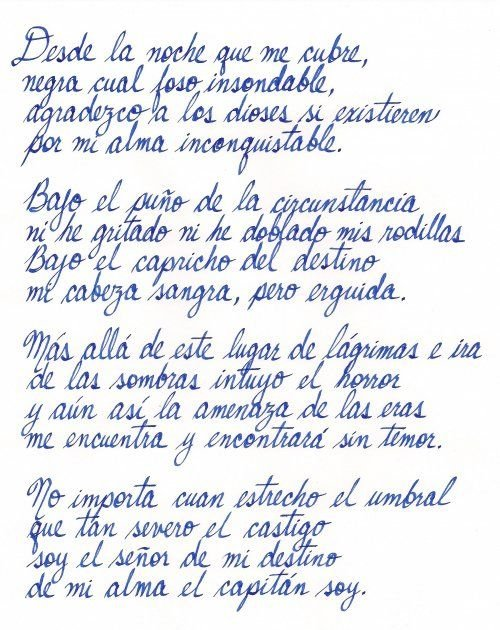
\includegraphics[width=\textwidth]{Graphics/antes_manuscrito.png}
		\caption{Facsimilar de entrada.}
		\label{fig:ocr-antes}
	\end{subfigure}
	\hfill
	\begin{subfigure}[t]{0.48\textwidth}
		\centering
		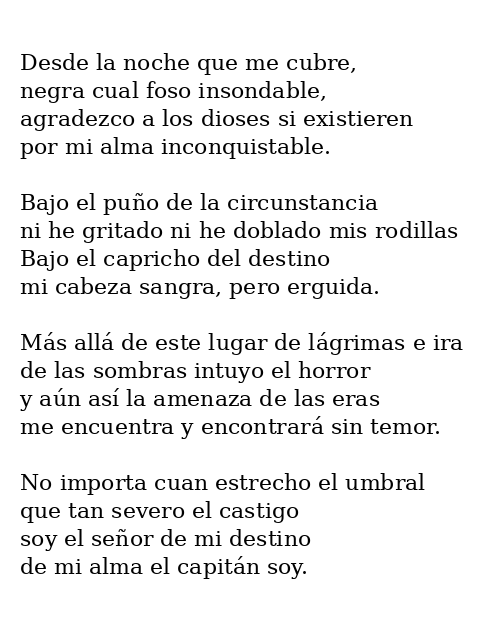
\includegraphics[width=\textwidth]{Graphics/despues_transcripcion.png}
		\caption{Transcripción producida.}
		\label{fig:ocr-despues}
	\end{subfigure}
	\caption{Comparación entre un facsimilar de entrada y la transcripción producida por un sistema OCR.}
	\label{fig:ocr-antes-despues}
\end{figure}

Cuando la imagen procede de la digitalización de un documento físico, recibe el nombre de facsimilar. Un facsimilar es una reproducción digital que preserva la apariencia visual completa del soporte: disposición de la página, tipografía, manchas, deterioro y demás características físicas. A diferencia de una transcripción, que representa únicamente el contenido textual, el facsimilar conserva la dimensión material del documento. El sistema de esta tesis opera sobre facsimilares como entrada.

El flujo de procesamiento de un sistema OCR moderno se descompone en cuatro etapas. La primera etapa es el preprocesamiento, que transforma la imagen de entrada en una representación normalizada mediante corrección de inclinación, eliminación de ruido y binarización. La segunda etapa es el análisis de diseño de página, que identifica las regiones de texto, las separa de figuras y márgenes, y detecta columnas y párrafos. La tercera etapa es el reconocimiento, durante la cual un modelo de aprendizaje automático produce la transcripción del texto de cada región o línea. La cuarta etapa es el postprocesado, que puede incluir corrección ortográfica o integración del texto en una base de datos. La figura~\ref{fig:ocr-etapas} muestra una misma imagen tras cada una de las cuatro etapas del flujo.

\begin{figure}[!htbp]
	\centering
	\begin{subfigure}[t]{0.40\textwidth}
		\centering
		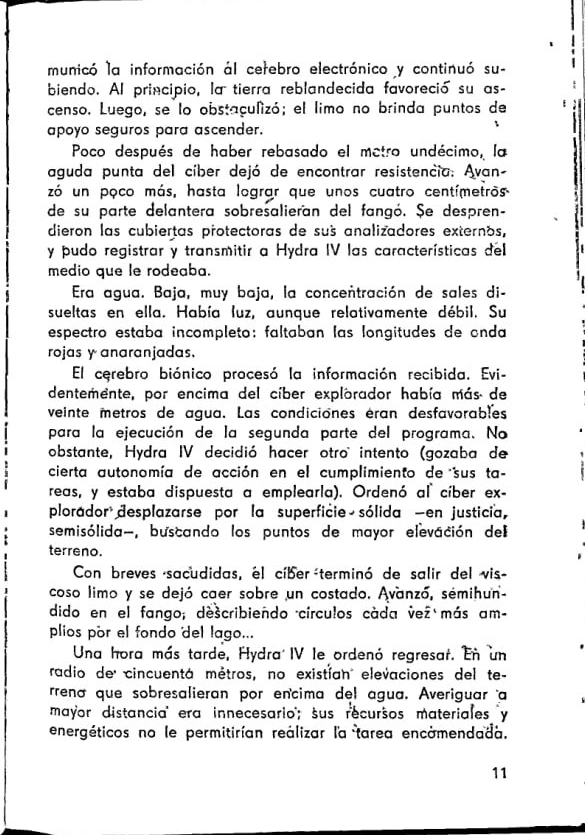
\includegraphics[width=\textwidth]{Graphics/etapa1_original.png}
		\caption{Imagen original.}
		\label{fig:etapa1}
	\end{subfigure}
	\hfill
	\begin{subfigure}[t]{0.40\textwidth}
		\centering
		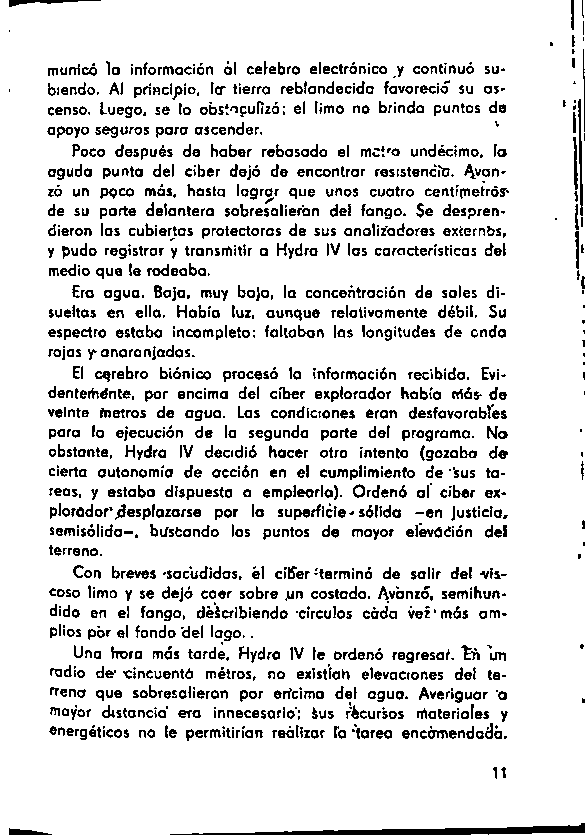
\includegraphics[width=\textwidth]{Graphics/etapa2_binarizada.png}
		\caption{Tras preprocesamiento.}
		\label{fig:etapa2}
	\end{subfigure}
	
	\vspace{0.3em}
	
	\begin{subfigure}[t]{0.40\textwidth}
		\centering
		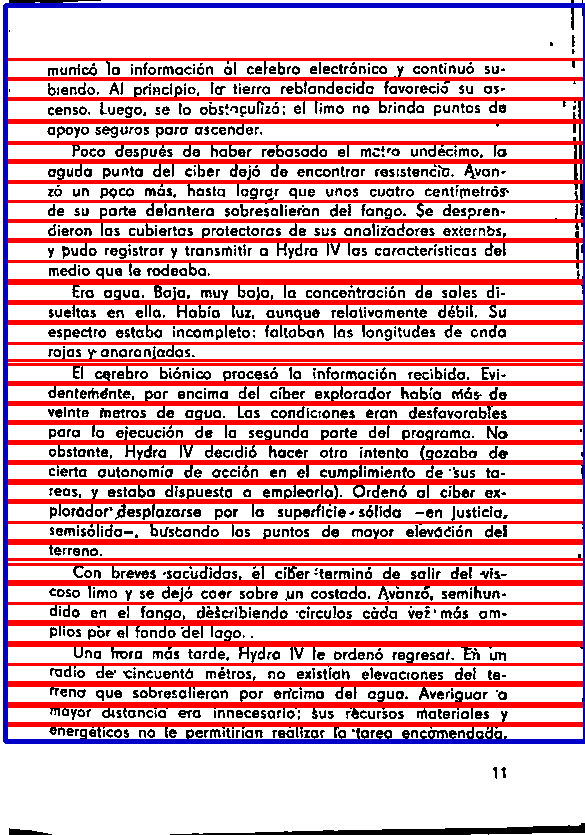
\includegraphics[width=\textwidth]{Graphics/etapa3_diseno.png}
		\caption{Tras análisis de diseño.}
		\label{fig:etapa3}
	\end{subfigure}
	\hfill
	\begin{subfigure}[t]{0.40\textwidth}
		\centering
		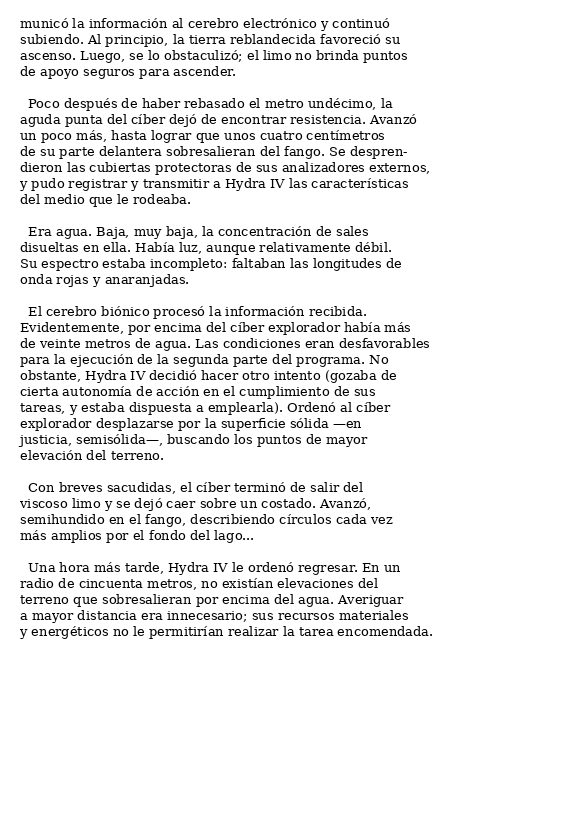
\includegraphics[width=\textwidth]{Graphics/etapa4_transcripcion.png}
		\caption{Tras reconocimiento.}
		\label{fig:etapa4}
	\end{subfigure}
	\caption{Misma página de un documento tras cada una de las cuatro etapas del flujo de procesamiento OCR.}
	\label{fig:ocr-etapas}
\end{figure}

El sistema construye las etapas de preprocesamiento y reconocimiento para documentos impresos en español. La descripción del flujo completo permite situar cada componente dentro de un marco arquitectónico de referencia. La siguiente subsección introduce dos variantes de OCR que trabajan sobre unidades de texto distintas: el OCR de caracteres aislados y el OCR de líneas completas. La decisión de cuál variante elegir determina la arquitectura que el reconocedor adopta.

\subsection{OCR de caracteres aislados frente a OCR de líneas completas}
\label{subsec:enfoques-ocr}

El enfoque clásico del OCR segmenta la imagen en caracteres individuales y clasifica cada carácter de forma independiente. El método exige que la segmentación sea perfecta. Si dos caracteres se tocan o si la separación es ambigua, el clasificador no recibe información suficiente para resolver el caso~\cite{smith2007tesseract,subramani2021survey}. Al procesar cada carácter en aislamiento, el modelo no incorpora la relación entre el carácter y sus vecinos. La consecuencia es que ciertas ambigüedades tipográficas resultan irresolubles. La secuencia ``rn'' en una fuente deteriorada, por ejemplo, puede ser visualmente indistinguible de la letra ``m'' vista en solitario, y un clasificador de caracteres aislados no posee los mecanismos para desambiguar.

El enfoque moderno toma una línea de texto completa como unidad de entrada y produce la secuencia de caracteres correspondiente en una sola pasada, sin segmentación previa. La elección justifica la arquitectura CRNN+CTC que propone Shi et al. en 2016~\cite{shi2016crnn}, que evita la segmentación explícita y aprovecha el contexto de la línea durante el reconocimiento. En el sistema para el centro de investigaciones culturales se adopta el enfoque moderno por razones que se desarrollan en el capítulo~\ref{chap:modelo}.

% -----------------------------------------------------------------------------
\section{Fundamentos de redes neuronales y aprendizaje supervisado}
\label{sec:redes-neuronales}

El sistema emplea un modelo de reconocimiento que se sustenta en redes neuronales profundas entrenadas con paradigma supervisado. La sección expone los conceptos necesarios para comprender el diseño y el funcionamiento del modelo: qué es una red neuronal artificial, en qué consiste el entrenamiento supervisado y qué es el sobreajuste.

\subsection{Redes neuronales artificiales y entrenamiento}

Una red neuronal artificial es una función paramétrica compuesta por capas de unidades de cómputo llamadas neuronas, con pesos ajustables. Cada neurona recibe una combinación lineal de las salidas de la capa anterior, aplica una función de activación no lineal y propaga el resultado a la capa siguiente. La composición de capas permite representar funciones progresivamente más abstractas de los datos de entrada~\cite{goodfellow2016deeplearning}.

El entrenamiento de la red consiste en encontrar valores de los pesos que minimizan una función de pérdida. La función mide la discrepancia entre la salida que la red produce y la salida esperada sobre un conjunto de ejemplos. La minimización opera mediante retropropagación. El algoritmo calcula el gradiente de la pérdida respecto a cada peso. A continuación, actualiza cada peso en la dirección que reduce el gradiente. El proceso itera durante múltiples pasadas sobre el \textit{corpus} de entrenamiento, y una vez concluido, los pesos condensan la información que la red extrae del \textit{corpus}. Este documento propone un sistema en el que los pesos del modelo codifican la correspondencia entre imágenes de líneas de texto y sus transcripciones.

\subsection{Aprendizaje supervisado y conjuntos de datos}

Un conjunto de datos de entrenamiento supervisado es una colección de pares en la que cada par está formado por una entrada y una etiqueta que un humano o un proceso controlado asigna~\cite{goodfellow2016deeplearning}. En el contexto del proyecto que este documento propone, cada par está formado por una imagen de una línea de texto y su transcripción exacta. El \textit{corpus} resulta supervisado porque las etiquetas resultan ciertas desde el momento en que el generador produce la imagen, lo que elimina la necesidad de anotación manual posterior.

La diversidad de los pares y la representatividad de su distribución respecto al problema real determinan la capacidad de generalización del modelo. Un \textit{corpus} reducido o sesgado produce modelos que rinden bien en el conjunto de entrenamiento pero fallan en datos nuevos. La consideración condiciona directamente las decisiones de diseño del \textit{corpus} sintético que el capítulo~\ref{chap:corpus} presenta.

\subsection{Sobreajuste y generalización}\label{subsec:sobreajuste}

El sobreajuste, conocido en la literatura como \textit{overfitting}, ocurre cuando el modelo memoriza los datos de entrenamiento en lugar de extraer patrones generalizables. Un modelo sobreajustado obtiene resultados excelentes sobre los ejemplos vistos durante el entrenamiento, pero falla en datos nuevos al no capturar los patrones subyacentes~\cite{goodfellow2016deeplearning}.

En el contexto del proyecto, el riesgo de sobreajuste se manifiesta en la selección de fuentes tipográficas para el \textit{corpus} sintético. El uso de cientos de fuentes con alta redundancia visual no aporta variabilidad efectiva pero multiplica los ejemplos con patrones equivalentes, lo cual empuja al modelo a memorizarlos~\cite{goodfellow2016deeplearning,shorten2019augmentation}. Por la misma razón se prefirió un conjunto pequeño de fuentes con diversidad estilística. Los detalles de la decisión se desarrollan en el capítulo~\ref{chap:corpus}.

% -----------------------------------------------------------------------------
\section{Propiedades estadísticas del lenguaje natural}
\label{sec:lenguaje}

El diseño del \textit{corpus} de entrenamiento descansa sobre una propiedad estadística del lenguaje natural: la distribución de frecuencias de los caracteres. En texto natural, la frecuencia de aparición de los elementos sigue una distribución de potencia~\cite{zipf1949human}. Algunos elementos concentran la mayoría de las ocurrencias, mientras que el resto resultan infrecuentes. El fenómeno se manifiesta tanto a nivel de palabras como a nivel de caracteres y sílabas.

En español, las vocales no acentuadas y unas pocas consonantes frecuentes concentran la mayor parte de las apariciones en un texto corrido. Símbolos como la raya de diálogo, las comillas angulares, los corchetes o el signo de porcentaje resultan infrecuentes en la misma medida. Un modelo que aprende sobre datos con distribución natural tenderá a reconocer correctamente las vocales y fallará en los símbolos raros por insuficiencia de ejemplos. El capítulo~\ref{chap:corpus} describe una estrategia para evitar las asimetrías por sobremuestreo. Con la propiedad estadística establecida, las siguientes secciones introducen las herramientas que miden el rendimiento del sistema y los trabajos similares que sustentan la propuesta.

% -----------------------------------------------------------------------------
\section{Métricas de evaluación de sistemas OCR}
\label{sec:metricas}

La evaluación de un sistema OCR requiere métricas que cuantifiquen la similitud entre la transcripción producida por el modelo y la transcripción de referencia. La sección define primero las métricas generales de clasificación que sustentan el vocabulario conceptual del campo, y a continuación introduce las métricas específicas del reconocimiento de secuencias.

\subsection{Precisión, recall y F1}

En clasificación, la precisión mide la proporción de predicciones positivas del modelo que resultan correctas:

\begin{equation}
	P = \frac{VP}{VP + FP},
	\label{eq:precision}
\end{equation}

donde $VP$ son los verdaderos positivos y $FP$ los falsos positivos. El \textit{recall}, llamado también sensibilidad, mide la proporción de casos positivos reales detectados por el modelo:

\begin{equation}
	R = \frac{VP}{VP + FN},
	\label{eq:recall}
\end{equation}

donde $FN$ son los falsos negativos. La medida F1 es la media armónica de precisión y recall, y combina ambas en un solo número:

\begin{equation}
	F_1 = \frac{2 \cdot P \cdot R}{P + R}.
	\label{eq:f1}
\end{equation}

Existe una compensación inherente entre precisión y recall. Un modelo restrictivo alcanza alta precisión a costa de un recall bajo. Un modelo permisivo presenta el comportamiento opuesto. La F1 equilibra ambos extremos y resulta útil cuando el problema demanda una métrica única. Las tres definiciones no resultan directamente aplicables al OCR de secuencias, pero constituyen el vocabulario conceptual sobre el cual el campo construye sus métricas específicas.

\subsection{Tasa de error de carácter, tasa de error de palabra y exactitud por línea}

La tasa de error de carácter, conocida por sus siglas inglesas CER, del término \textit{Character Error Rate}~\cite{jurafsky2024slp}, mide la proporción de caracteres incorrectos en la transcripción respecto a la transcripción de referencia. Se calcula mediante la distancia de Levenshtein a nivel de carácter, normalizada por la longitud de la referencia:

\begin{equation}
	CER = \frac{S_c + I_c + D_c}{N_c},
	\label{eq:cer}
\end{equation}

donde $S_c$, $I_c$ y $D_c$ son los números de sustituciones, inserciones y eliminaciones de caracteres, y $N_c$ es el número total de caracteres de la referencia. La métrica satisface $0 \leq \mathrm{CER} \leq 1$, donde un CER de~0 corresponde a una transcripción perfecta y un CER de~1 indica un número de errores igual al número de caracteres del texto de referencia.

La tasa de error de palabra, denominada WER, del término \textit{Word Error Rate}~\cite{jurafsky2024slp}, es análoga al CER pero a nivel de palabras:

\begin{equation}
	WER = \frac{S_w + I_w + D_w}{N_w}.
	\label{eq:wer}
\end{equation}

El WER es más exigente que el CER porque un solo carácter incorrecto dentro de una palabra cuenta como un error de palabra completo. La diferencia hace al WER sensible a errores que distorsionan el significado léxico, y menos informativo sobre errores aislados en caracteres especiales.

La exactitud por línea~\cite{jurafsky2024slp} es la métrica más exigente de las tres. Mide la proporción de líneas de texto donde la transcripción coincide exactamente con la referencia, sin ningún error:

\begin{equation}
	\mathrm{LineAcc} = \frac{\text{líneas sin error}}{\text{total de líneas}}.
	\label{eq:lineacc}
\end{equation}

Una sola sustitución en cualquier posición de la línea la marca como incorrecta. La métrica resulta útil para evaluar la viabilidad del sistema en casos de uso donde no se admite intervención humana posterior. Las tres métricas, tomadas en conjunto, ofrecen una visión complementaria del rendimiento. El CER informa sobre la tasa de error tipográfico, el WER sobre la integridad léxica y la exactitud por línea sobre la viabilidad para automatización completa. Con el vocabulario de evaluación definido, la siguiente sección revisa los trabajos previos que abordan problemas equivalentes al planteado en la tesis.

% -----------------------------------------------------------------------------
\section{Estado del arte}
\label{sec:estado-arte}

Esta sección sintetiza los trabajos previos sobre los que se apoya el desarrollo del sistema. La revisión se organiza por bloques temáticos. El primero presenta los motores OCR clásicos de código abierto. El segundo aborda las arquitecturas basadas en aprendizaje profundo con función de pérdida \textit{Connectionist Temporal Classification}, conocida por sus siglas inglesas CTC~\cite{graves2006ctc}. El tercero recoge las propuestas basadas en \textit{transformers}~\cite{vaswani2017transformer}. El cuarto trata la generación sintética de datos para OCR. El quinto introduce las plataformas de digitalización documental de uso institucional. El sexto cierra con los trabajos específicos para texto impreso en español.

\subsection{Motores OCR clásicos: Tesseract y Calamari}

Tesseract es un motor OCR de código abierto, distribuido bajo licencia Apache~2.0. Lo desarrolló originalmente Hewlett-Packard entre los años ochenta y noventa, y entre 2006 y agosto de 2017 lo mantuvo Google~\cite{smith2007tesseract}. Desde esa fecha el desarrollo lo continúa la comunidad de código abierto a través del repositorio público del proyecto. El motor admite más de~100 idiomas y dispone de paquetes de datos entrenados para el reconocimiento. A partir de su versión~4, el reconocedor interno de Tesseract es una red neuronal basada en LSTM. La arquitectura sitúa al motor en la familia de las soluciones con función de pérdida CTC~\cite{graves2006ctc}.

Calamari, presentado por Wick et al.~\cite{wick2018calamari}, es un motor OCR de código abierto especializado en el reconocimiento de líneas de texto, con énfasis en documentos impresos históricos. La arquitectura central de Calamari combina una red convolucional~\cite{goodfellow2016deeplearning} con una red recurrente bidireccional~\cite{goodfellow2016deeplearning} y una capa CTC, esquema equivalente al de la CRNN~\cite{shi2016crnn}. El motor ha alcanzado popularidad en el ámbito de las humanidades digitales por su capacidad para procesar tipografías históricas como la \textit{Fraktur}~\cite{breuel2013ocropus}.

Ambos motores ofrecen reconocimiento listo para uso, pero presentan limitaciones para el problema que motiva a esta tesis. Tesseract dispone de un modelo para el español de propósito general, sin adaptación a la distribución de caracteres ni al perfil tipográfico de un dominio documental específico. Calamari requiere conjuntos de datos con anotación humana específicos para cada dominio. En el capítulo~\ref{chap:corpus} se ofrece una justificación a detalle de la decisión de desarrollar un \textit{corpus} propio.

\subsection{Arquitecturas basadas en aprendizaje profundo: CRNN + CTC}
\label{subsec:crnn-ctc-arte}

El trabajo de Shi, Bai y Yao~\cite{shi2016crnn} propuso en~2016 la arquitectura CRNN, que combina una red neuronal convolucional con una red neuronal recurrente bidireccional, y que la función de pérdida \textit{Connectionist Temporal Classification}, CTC por sus siglas en inglés, entrena. La arquitectura transcribe líneas de texto completas sin segmentación previa de caracteres, y como describe la sección~\ref{subsec:enfoques-ocr}, esta propiedad la sitúa en el enfoque moderno. Graves et al.~\cite{graves2006ctc} introdujeron por primera vez la función CTC para el reconocimiento de habla, y permite entrenar redes que producen secuencias de longitud variable sin alineamiento explícito entre entrada y salida.

El trabajo de Breuel et al.~\cite{breuel2013ocropus} demostró en~2013 que una red bidireccional LSTM, sin modelo de lenguaje ni postprocesado, alcanza tasas de error inferiores al~2\,\% sobre texto impreso en inglés y sobre Fraktur degradada artificialmente. El resultado estableció la viabilidad de las arquitecturas LSTM para el reconocimiento de líneas impresas, y abrió la puerta al entrenamiento sobre \textit{corpus} con artefactos sintéticos que reproducen las condiciones visuales de los documentos objetivo.

La arquitectura CRNN+CTC presenta dos propiedades que la convierten en la opción preferida para el sistema. Primero, permite explotar el contexto oracional durante el reconocimiento, lo cual desambigua errores tipográficos que un clasificador de caracteres aislados no puede resolver. Segundo, su entrenamiento sobre líneas completas se ajusta al formato del \textit{corpus} sintético generado. Las decisiones de diseño del modelo concreto se exponen en el capítulo~\ref{chap:modelo}.

\subsection{Arquitecturas basadas en transformers: TrOCR y derivados}

A partir de la introducción de la arquitectura \textit{Transformer} por Vaswani et al.~\cite{vaswani2017transformer} en~2017, el aprendizaje profundo aplicado a tareas de lenguaje y visión adoptó el mecanismo de atención de forma generalizada. En el campo del reconocimiento óptico de caracteres, el trabajo de Li et al.~\cite{li2021trocr} propuso en~2021 la arquitectura TrOCR, que reemplaza por completo el esquema CNN+RNN. Como codificador de imagen emplea un \textit{Vision Transformer}, y como decodificador un \textit{transformer} de texto. El modelo se entrena con un esquema de preentrenamiento sobre datos sintéticos seguido de \textit{fine-tuning} sobre datos reales.

El trabajo de Laurent y Lauar~\cite{laurent2024spanishtrocr} adaptó TrOCR al español mediante \textit{fine-tuning} desde el punto de control en inglés. El trabajo concluye que el \textit{fine-tuning} desde un modelo en inglés produce mejores resultados que el entrenamiento de un decodificador específico para el español. La estrategia exige infraestructura computacional mayor que la CRNN+CTC para alcanzar mejoras marginales sobre tipografías de imprenta estándar, donde la arquitectura CRNN ya rinde por debajo del~2\,\% de CER. La consideración sustenta la elección de CRNN+CTC para el sistema descrito en la tesis, justificada en detalle en el capítulo~\ref{chap:modelo}.

\subsection{Generación sintética de datos para OCR}

El trabajo de Jaderberg et al.~\cite{jaderberg2014synthetic} demostró en~2014 que el entrenamiento de redes neuronales sobre datos sintéticos puede sustituir el uso de datos reales en escenarios de reconocimiento de texto natural. Los modelos resultantes alcanzan tasas de error competitivas con \textit{corpus} generados enteramente por procesos automáticos. La demostración estableció la generación sintética como una alternativa viable cuando los datos con anotación humana son escasos o inexistentes para el idioma objetivo.

Trabajos posteriores extendieron la idea a configuraciones específicas. Etter et al.~\cite{etter2019synthrecipe} describieron un protocolo de generación sintética para sistemas OCR de líneas completas, con énfasis en la diversidad tipográfica y en los artefactos del escaneo real. La línea de trabajo más cercana al proyecto que esta tesis describe es la de Laurent y Lauar~\cite{laurent2024spanishtrocr}, que generó un \textit{corpus} de dos millones de muestras para entrenar TrOCR en español a partir de páginas web de la Wikipedia hispanoamericana.

El sistema que esta tesis presenta entrena con datos que el procedimiento produce de manera similar a la que el estado del arte describe, con dos diferencias al respecto. Primero, el generador toma el \textit{corpus} de obras literarias del dominio público en lugar de texto extraído de la web. La elección asegura riqueza léxica y densidad de signos tipográficos propios del español formal. Segundo, una estrategia explícita de sobremuestreo por grupos equilibra las frecuencias de caracteres, en lugar de una distribución uniforme o de la distribución natural del \textit{corpus} base. El capítulo~\ref{chap:corpus} desarrolla la justificación de ambas decisiones.

\subsection{Plataformas de digitalización documental: Transkribus}

Muehlberger et al.~\cite{muehlberger2019transkribus} describen Transkribus, plataforma para el reconocimiento, transcripción y búsqueda de documentos históricos. La cooperativa READ-COOP mantiene la plataforma actualmente, desarrollada en el marco del proyecto europeo \textit{Recognition and Enrichment of Archival Documents}, conocido por sus siglas READ. La plataforma integra motores de reconocimiento de texto manuscrito y OCR para impresos junto con herramientas de gestión, búsqueda y revisión colaborativa de transcripciones. Cuenta con una comunidad consolidada de decenas de miles de usuarios registrados.

Transkribus constituye la referencia funcional más cercana al sistema que este trabajo aspira a desarrollar. Integra el flujo completo, desde la subida del facsimilar hasta la corrección de la transcripción mediante un editor colaborativo. El capítulo~\ref{chap:web} presenta una aplicación que adopta un esquema funcional similar a Transkribus, adaptado al contexto del Instituto Juan Marinello y a la integración de modelos OCR para el idioma español.

\subsection{Trabajos previos sobre OCR para texto impreso en español}

La literatura específica sobre OCR para texto impreso en español es escasa. La mayor parte de los recursos disponibles asumen el idioma inglés y, en menor medida, otros idiomas con presencia mayoritaria en los conjuntos de datos públicos~\cite{laurent2024spanishtrocr}. El conjunto de competiciones internacionales \textit{Robust Reading Competition on Multi-lingual Scene Text} de ICDAR~\cite{nayef2019icdarmlt}, referencia metodológica del campo, contempla diez lenguas en su edición de~2019: el chino, el japonés, el coreano, el inglés, el francés, el árabe, el italiano, el alemán, el bangla y el devanagari. La ausencia del español del conjunto es ilustrativa del estado del arte en el campo. El trabajo de Laurent y Lauar~\cite{laurent2024spanishtrocr} constituye una de las primeras propuestas dedicadas explícitamente al español, y limita su evaluación a documentos del tipo \textit{Visual Rich Document}~\cite{laurent2024spanishtrocr}, con presencia frecuente de formularios y campos estructurados.


Los \textit{datasets} de uso común en investigación OCR omiten signos frecuentes en documentos formales en español. Entre los signos ausentes están la raya de diálogo, las comillas angulares, los signos de apertura de interrogación y exclamación, la eñe y las vocales acentuadas. Un modelo que aprende sobre vocabularios incompletos resulta incapaz de transcribir correctamente los documentos formales en español que motivan el trabajo. El capítulo~\ref{chap:corpus} presenta el análisis sistemático de los \textit{datasets} existentes, junto con la justificación del desarrollo de un \textit{corpus} propio.


% -----------------------------------------------------------------------------
\section{Tecnologías para el desarrollo de la aplicación web}
\label{sec:tecnologias-web}

Para comodidad del usuario final, el desarrollo de esta tesis incorpora una aplicación web que el capítulo~\ref{chap:web} describe. Esta aplicación, que permite usar las funcionalidades del sistema de manera fácil, descansa sobre un conjunto de tecnologías abiertas que proyectos similares emplean ampliamente. La sección introduce el \textit{framework} de desarrollo y los mecanismos de persistencia. La descripción detallada de las decisiones de arquitectura espera al capítulo correspondiente.

\subsection{Django y el patrón Modelo-Vista-Plantilla}\label{subsec:django-mvt}

Django es un \textit{framework} de desarrollo web en Python, distribuido bajo licencia BSD~\cite{osi-bsd}. Está diseñado en torno al patrón Modelo-Vista-Plantilla, conocido por sus siglas MVT, del término inglés \textit{Model-View-Template}~\cite{django-mvt}. El patrón separa la lógica de los datos en los modelos, la lógica de presentación en las plantillas, y la lógica de control en las vistas. La separación facilita el mantenimiento del código y la división del trabajo entre componentes. La figura~\ref{fig:mvt-diagrama} resume las relaciones entre los cuatro elementos del patrón.

\begin{figure}[!htbp]
	\centering
	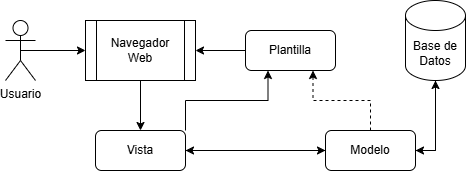
\includegraphics[width=0.78\textwidth]{Graphics/mvt_diagrama.png}
	\caption{Patrón Modelo-Vista-Plantilla de Django. El navegador del usuario envía una petición a la vista, que consulta el modelo cuando necesita datos persistentes; el modelo intermedia con la base de datos. La vista pasa los datos a la plantilla, que produce la respuesta HTML que el navegador recibe.}
	\label{fig:mvt-diagrama}
\end{figure}

Django ofrece una infraestructura integrada de correspondencia objeto-relacional, conocida por sus siglas ORM del término inglés \textit{Object-Relational Mapping}, un sistema de migraciones automatizado, un mecanismo declarativo de formularios y una infraestructura de autenticación con roles y permisos. La combinación reduce la cantidad de código necesario para implementar las funcionalidades comunes de una aplicación web. El esfuerzo de desarrollo se concentra entonces en los componentes específicos del problema, como la integración del modelo de OCR y el editor de doble panel para la revisión de transcripciones.

\subsection{Persistencia: PostgreSQL y XML}

La aplicación utiliza dos mecanismos de persistencia complementarios. Los metadatos estructurados de los documentos se almacenan en una base de datos relacional PostgreSQL~\cite{postgresql}. Las transcripciones, que combinan texto plano con regiones definidas por el usuario y referencias a páginas, se almacenan en ficheros XML, uno por cada página.

La decisión responde a dos consideraciones. La primera es la legibilidad humana directa. Un revisor puede abrir el fichero XML con un editor de texto e interpretar y modificar la transcripción sin herramientas auxiliares. La segunda es la posibilidad de convertir las transcripciones a estándares mayores como ALTO~\cite{loc-alto}, PAGE-XML~\cite{pletschacher2010page} o TEI~\cite{tei-consortium}, en caso de que el archivo se integre en un repositorio institucional con requisitos de interoperabilidad. El esquema que el trabajo emplea constituye un subconjunto razonable de ALTO, lo que facilita la migración futura sin retrabajo. El capítulo~\ref{chap:web} describe a detalle el esquema y el modelo de datos relacional que el sistema utiliza.

% -----------------------------------------------------------------------------
% Transición al capítulo 2
% -----------------------------------------------------------------------------

Con la fundamentación teórica establecida, los antecedentes presentados y la metodología declarada, el capítulo cierra. El capítulo siguiente aborda la primera contribución técnica del trabajo: la generación del \textit{corpus} sintético de pares imagen--transcripción sobre el que se entrena el modelo de reconocimiento.
